\documentclass[10pt]{article}
\usepackage[english]{babel}
\usepackage{amsmath}
\usepackage{graphicx}
\usepackage[colorinlistoftodos]{todonotes}
\pagestyle{headings}
\usepackage{indentfirst}
\usepackage[utf8]{inputenc}
\usepackage{xeCJK}
\usepackage{float}
\usepackage {subcaption}

%% Code blocl setting
\usepackage{listings}
\renewcommand{\lstlistingname}{Code}% Listing -> Algorithm
\usepackage{color}

\definecolor{dkgreen}{rgb}{0,0.6,0}
\definecolor{gray}{rgb}{0.5,0.5,0.5}
\definecolor{mauve}{rgb}{0.58,0,0.82}

\lstset{frame=tb,
  language=Python,
  aboveskip=3mm,
  belowskip=3mm,
  showstringspaces=false,
  columns=flexible,
  basicstyle={\small\ttfamily},
  numbers=none,
  numberstyle=\tiny\color{gray},
  keywordstyle=\color{blue},
  commentstyle=\color{dkgreen},
  stringstyle=\color{mauve},
  breaklines=true,
  breakatwhitespace=true,
  tabsize=3
}

\begin{document}

\begin{titlepage}

\newcommand{\HRule}{\rule{\linewidth}{0.5mm}} % Defines a new command for the horizontal lines, change thickness here

\center % Center everything on the page

%----------------------------------------------------------------------------------------
%	HEADING SECTIONS
%----------------------------------------------------------------------------------------

\textsc{\LARGE Shanghai Jiaotong University}\\[1.5cm] % Name of your university/college
\textsc{\Large Big Data Processing Technology}\\[0.5cm] % Major heading such as course name
%\textsc{\large Minor Heading}\\[0.5cm] % Minor heading such as course title

%----------------------------------------------------------------------------------------
%	TITLE SECTION
%----------------------------------------------------------------------------------------

\HRule \\[0.4cm]
{ \huge \bfseries Project 1: Erasure Code in Hadoop}\\[0.4cm] % Title of your document
\HRule \\[1.5cm]

%----------------------------------------------------------------------------------------
%	AUTHOR SECTION
%----------------------------------------------------------------------------------------

\begin{minipage}{0.4\textwidth}
\begin{flushleft} \large
\emph{Author:}\\
% Your name
FEI Yixiao \\118260910031\\
LI Yanhao \\118260910036\\
LUO Dihao \\118260910039\\ % Your name
SHEN Shengyang \\118260910042\\
YAN Shuhan \\118260910050\\ % Your name
\end{flushleft}
\end{minipage}
~
\begin{minipage}{0.4\textwidth}
\begin{flushright} \large
\emph{Supervisor:} \\
Chentao  \textsc{WU} \\% Supervisor's Name
Xin  \textsc{XIE}
\end{flushright}
\end{minipage}\\[2cm]

% If you don't want a supervisor, uncomment the two lines below and remove the section above
%\Large \emph{Author:}\\
%John \textsc{Smith}\\[3cm] % Your name

%----------------------------------------------------------------------------------------
%	DATE SECTION
%----------------------------------------------------------------------------------------

{\large \today}\\[2cm] % Date, change the \today to a set date if you want to be precise

%----------------------------------------------------------------------------------------
%	LOGO SECTION
%----------------------------------------------------------------------------------------


\includegraphics[width=0.5\textwidth]{logo_SPEIT.jpg}\\[1cm] % Include a department/university logo - this will require the graphicx package

%----------------------------------------------------------------------------------------

\vfill % Fill the rest of the page with whitespace

\end{titlepage}
\indent
\section{Introduction:}
Erasure code is a method of data protection in which data is broken into fragments, expanded and encoded with redundant data pieces and stored across a set of different locations or storage media.

In hadoop system, an erasure code called RS code has already been implemented. For every \textbf{\textit{n}} data units, RS code will have \textbf{\textit{k}} parity units, which \textbf{\textit{k}} is set by user, and generate a matrix which size is $(\textbf{\textit{n}}+\textbf{\textit{k}})\times \textbf{\textit{n}}$, then store the data that has been transformed by this matrix. Although it will cost more disk space, when any data unit becomes unavailable, we could pick \textbf{\textit{n}} available units for reconstruction. We can pick these \textbf{\textit{n}} row in the matrix and calculate its inverse matrix, then multiply the vector to get the origin \textbf{\textit{n}} data unit.

But RS code has its disadvantage, each time we lost a unit, which is the most probable situation, we have to get all \textbf{\textit{n}} units for reconstruction, it's a huge cost of time, so maybe we could sacrifice some uncommonly occurred situation, for example lost \textbf{\textit{k}} units at the same time, to decrease the cost of most situation, for example lost only 1 unit.

LRC code is the solution for such situation, similar to RS code, LRC code also has \textbf{\textit{n}} data units and \textbf{\textit{k}} parity units, instead of RS code's \textbf{\textit{k}} parity units are related to every data unit, which we called global parity unit, LRC code has \textbf{\textit{l}} local parity units only related to certain data units, and \textbf{\textit{r}} global parity units where \textbf{\textit{l+r=k}}. In ours project, we choose $\textbf{\textit{n}}=6, \textbf{\textit{l}}=2, \textbf{\textit{r}}=2$. The structure shows in Figure 1. 


In the two local parity units, each is related to 3 data units, so that if any data unit is lost, we could use the other two data units and the related local parity unit for reconstruction. That only need half the data reading. Such method can'y handle the situation of four certain units lost, which the units are one local parity unit and the three data units it related to. But this situation is almost impossible to happen so the cost is nearly zero.

\begin{figure}[H]
\centerline{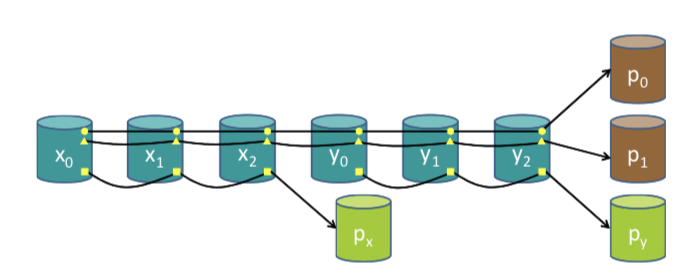
\includegraphics[width = 0.8\textwidth]{LRC-1.png}}
\caption{LRC structure}
%\label{fig_process}
\end{figure}

\section{Code:}
The implementation of LRC code is based on JAVA and composed with following files:
\begin{itemize}
\item LRCUtil.java: In this file we define the function to generate the encode matrix and the function to encode data. The encode matrix is composed by an $6\times 6$ identity matrix. Two local parity vectors, one with the first three elements are one and others are zero, another with the last three elements are one and others are zero. Two global parity vectors. All under GF($2^8$). The encode matrix shows as below:
$$
  \left[
  \begin{matrix}
   1 & 0 & 0 & 0 & 0 & 0 \\
   0 & 1 & 0 & 0 & 0 & 0 \\
   0 & 0 & 1 & 0 & 0 & 0 \\
   0 & 0 & 0 & 1 & 0 & 0 \\
   0 & 0 & 0 & 0 & 1 & 0 \\
   0 & 0 & 0 & 0 & 0 & 1 \\
   1 & 1 & 1 & 0 & 0 & 0 \\
   0 & 0 & 0 & 1 & 1 & 1 \\
   1 & 2 & 3 & 4 & 5 & 6 \\
   1 & 4 & 9 & 16 & 25 & 36 \\
  \end{matrix}
  \right]
$$
\item LRCRawErasureCoderFactory.java: In this file we declare the functions we need and merge the options into LRC code.
\item LRCRawEncoder.java: In this file we call the functions in LRCUtil.java to generate encode matrix and do the matrix multiplication to encode data.
\item LRCRawDecoder.java: In this file we recover the lost data. We separate the matrix into three parts:
\begin{itemize}
\item First local part: this part includes the first three data units and the related local parity unit.
\item Second local part: this part includes the other three data units and the related local parity unit.
\item Global part: this part includes the two global parity units.
\end{itemize}
Depend on different situation we will decode under following logic:
\begin{itemize}
\item One unit lost: If this unit belongs to the two local part, we will use the remaining three units to recover the lost unit. If it belongs to the global part, we will use the corresponding row of the encode matrix to re-calculate this unit.
\begin{figure}[H]
    \centering
    \begin{subfigure}[b]{0.5\textwidth}
        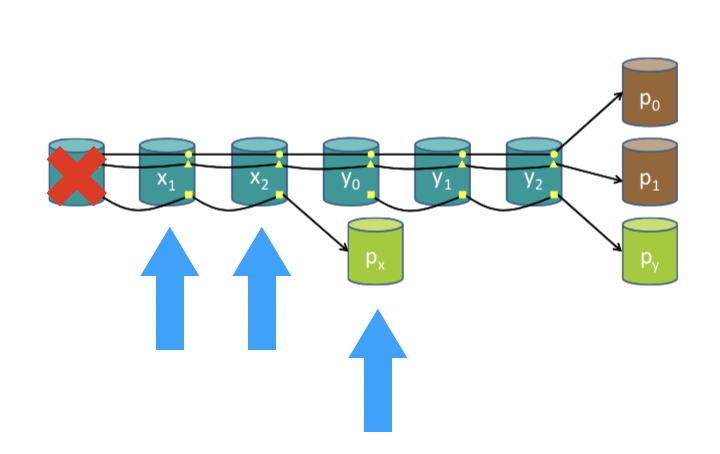
\includegraphics[width=\textwidth]{LRC-2.png}
        \caption{local unit lost}
%        \label{fig:visual_smap_o}
    \end{subfigure}
    
    \begin{subfigure}[b]{0.5\textwidth}
        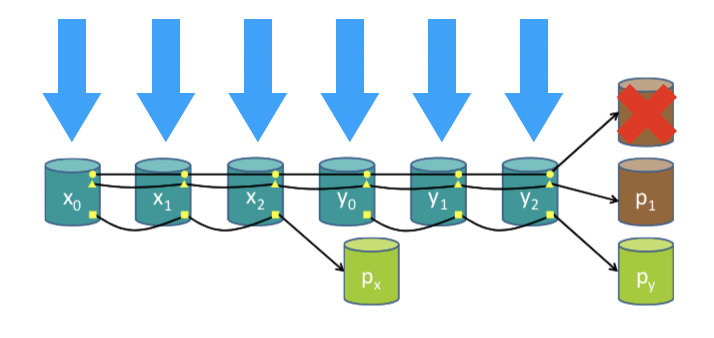
\includegraphics[width=\textwidth]{LRC-3.png}
        \caption{global unit lost}
  %      \label{fig:visual_smap_k}
    \end{subfigure}
%\label{fig_process}
\end{figure}
\item Two to four units lost: First we get which part does the first unit belong to and use the remaining units in this part, then use the global units if available, if the number of units still lower than 6, we randomly choose units in the last part.
\begin{figure}[H]
\centering
\begin{subfigure}[b]{0.5\textwidth}
        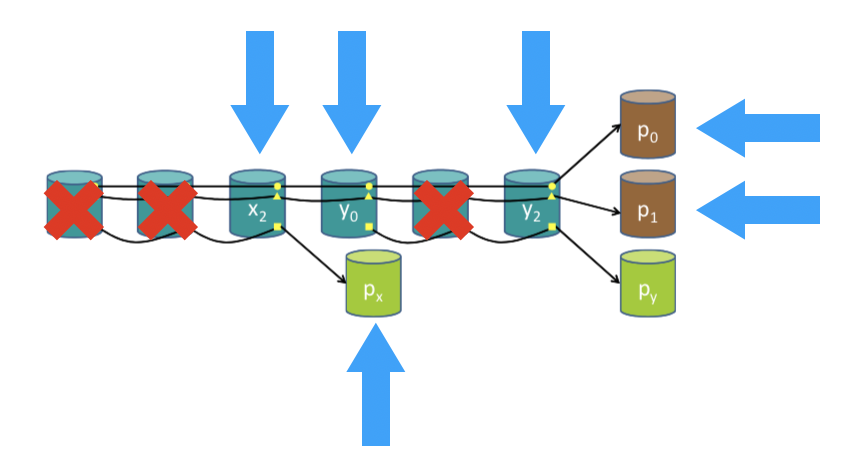
\includegraphics[width=\textwidth]{LRC-4.png}
        \caption{more than one unit lost}
%        \label{fig:visual_smap_o}
\end{subfigure}
\end{figure}

\item Four units in the same part lost or more than four units lost: This is the situation this LRC code can't recover.
\begin{figure}[H]
\centering
\begin{subfigure}[b]{0.5\textwidth}
        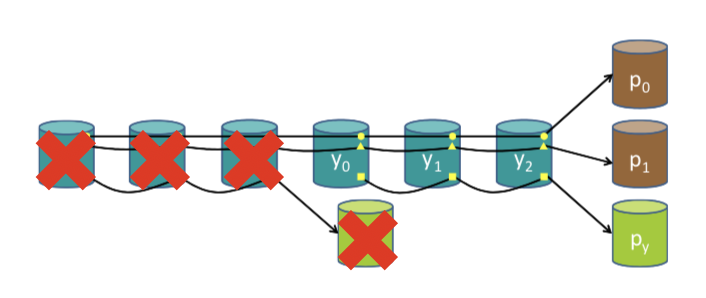
\includegraphics[width=\textwidth]{LRC-5.png}
        \caption{cannot recover}
%        \label{fig:visual_smap_o}
\end{subfigure}
\end{figure}
\end{itemize}
\end{itemize}

Using the above logic we get the decode matrix either $3 \times 3$ or $6\times 6$, then we calculate the invert matrix and recover the lost unit(s).



\section{Example}




% \begin{figure}[h]
% \centerline{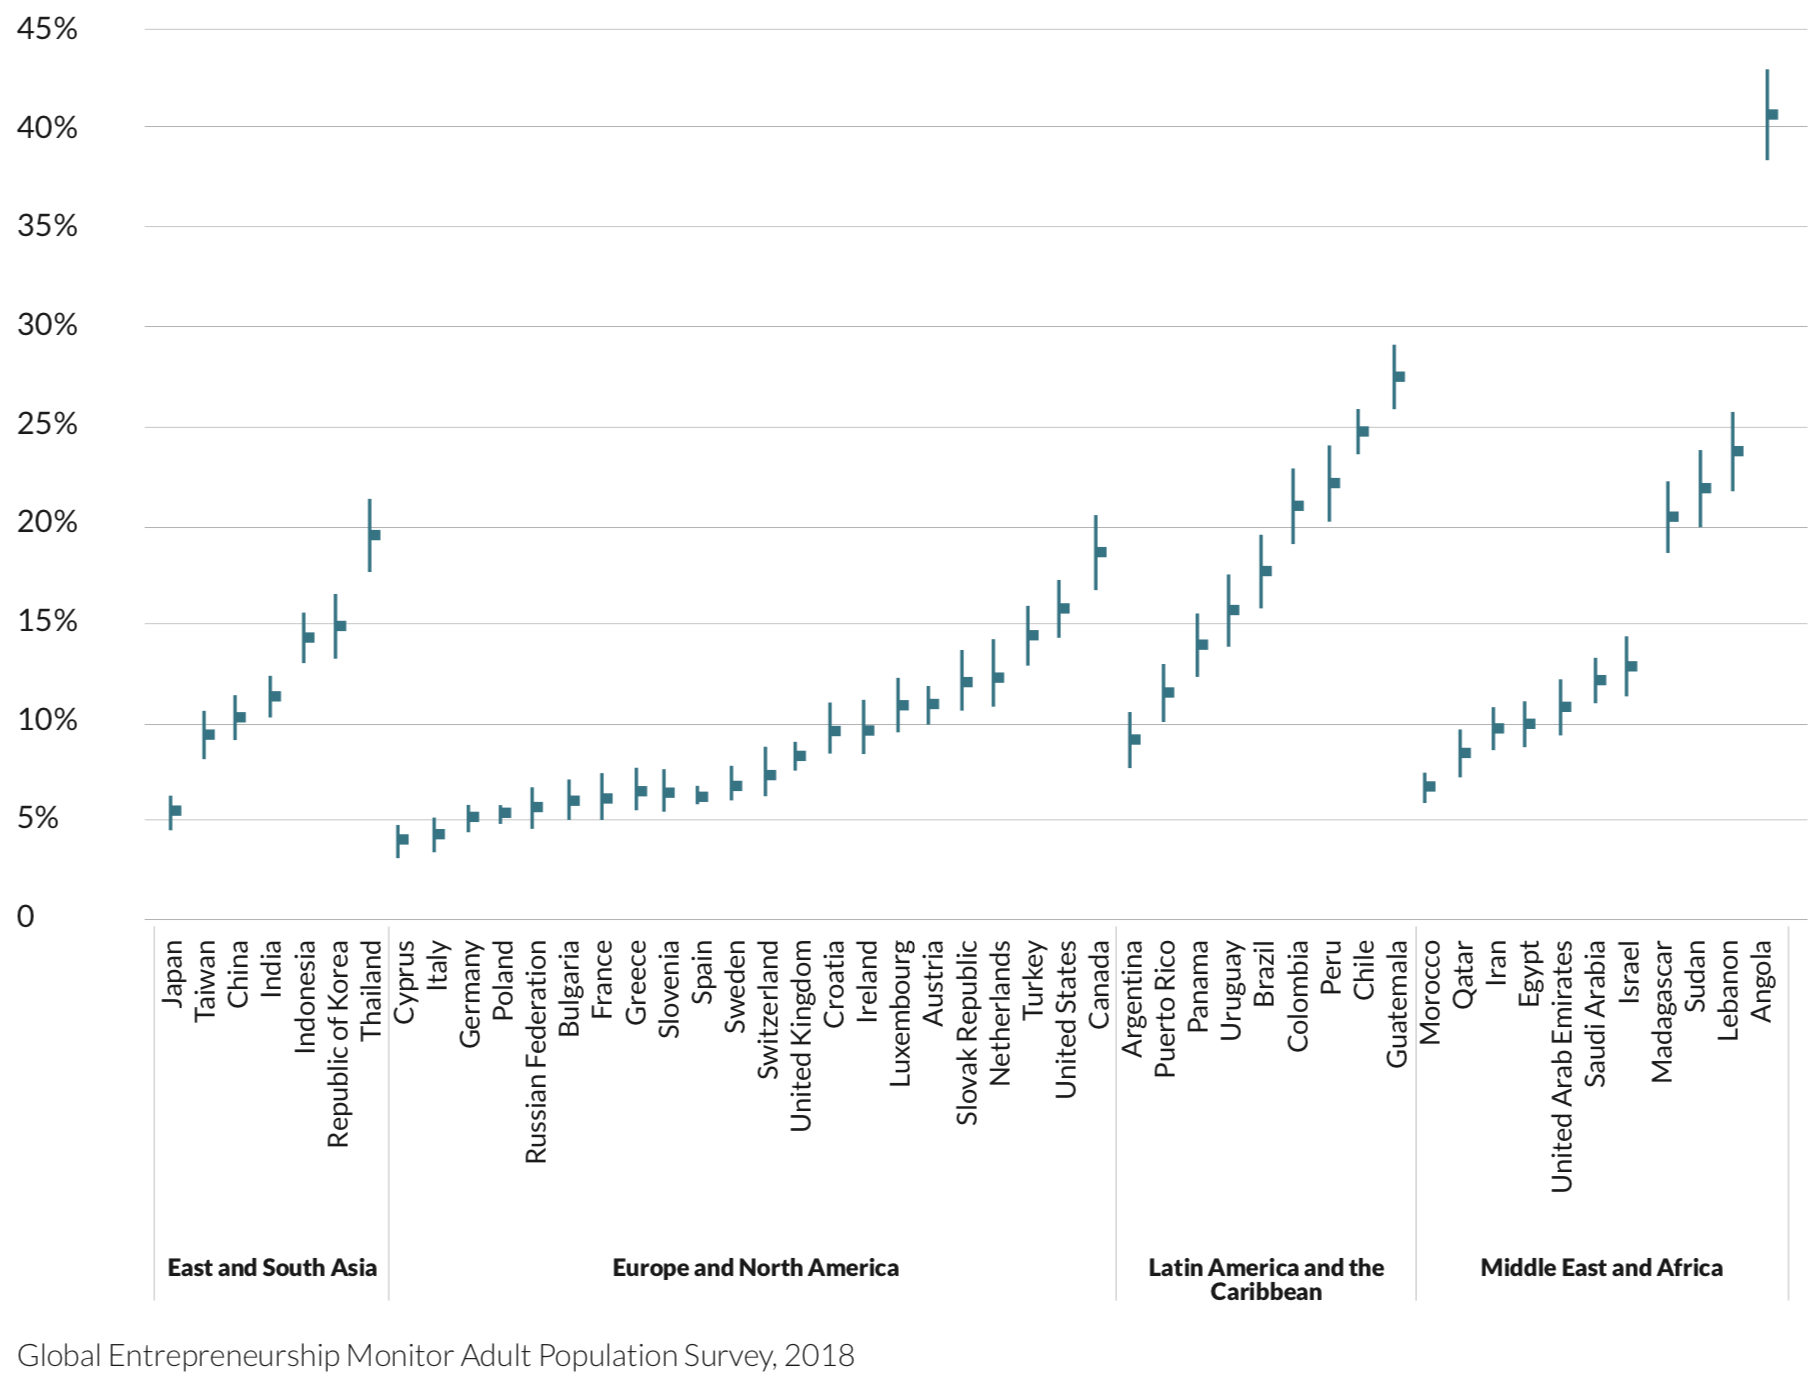
\includegraphics[width = 1\textwidth]{screenshot//2_2.png}}
% \caption{Total early-stage Entrepreneurial Activity (TEA) Rates among Adults (ages 18-64) in 487 Economies, in Four Geographic Regions}
% \label{fig_TEA_global}
% \end{figure}

% \section{Pod}
% \subsection{1 Pod with 1 Container}
%
% We can see after creating pod1 by pod1.yaml, we can execute any command by kubectl exec -it pod1 -- command.
%
% \begin{figure}[H]
% \centerline{\includegraphics[width = 0.7\textwidth]{screenshot//1.png}}
% \caption{1 Pod with 1 Container}
% % \label{fig_1pod1container}
% \end{figure}
%
% \subsection{1 Pod with 2 Containers}
%
% We can see after we change index.html in container ct-debian, we can also see the change in container ct-nginx.
%
% \begin{figure}[H]
% \centerline{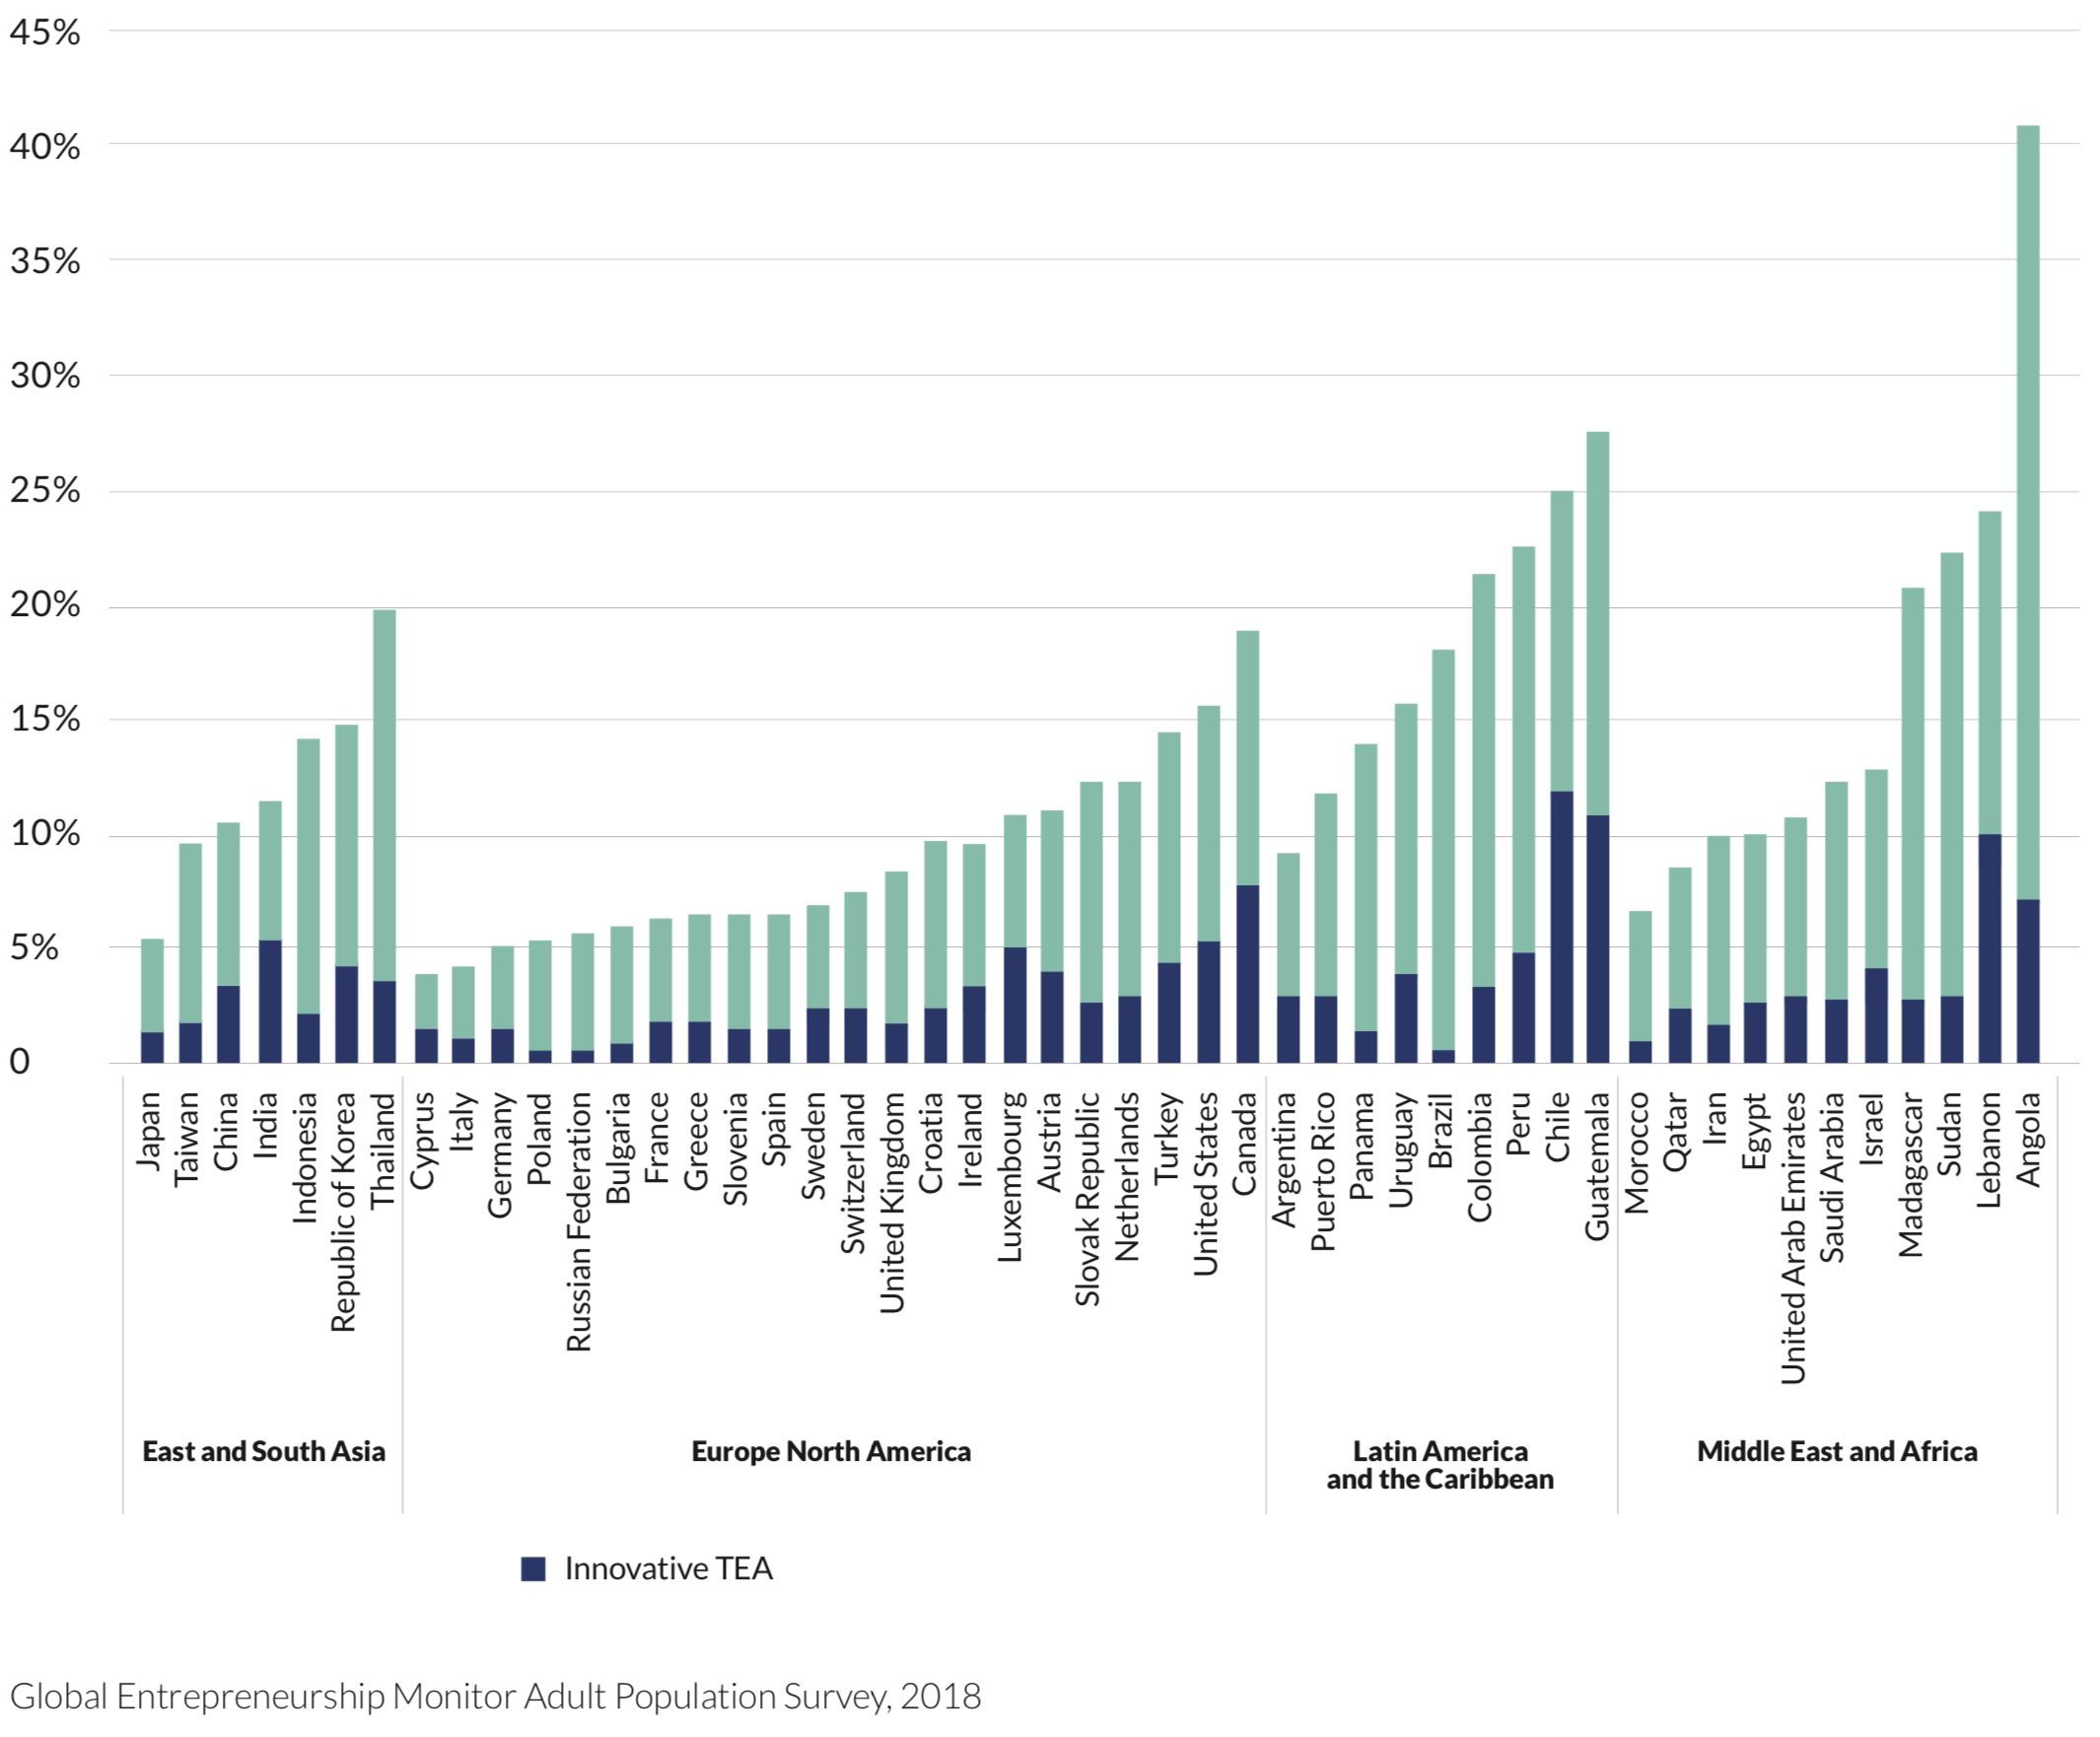
\includegraphics[width = 0.7\textwidth]{screenshot//2_1.png}}
% \caption{1 Pod with 2 Container}
% % \label{fig_1pod1container}
% \end{figure}






\end{document}
